
\chapter{Dinamica}
\minitoc

\section{\index{forza!fondamentale}Forze fondamentali}
\begin{itemize}
  \item forza gravitazionale
  \item forza elettromagnetica
  \item forza nucleare debole
  \item forza nucleare forte
\end{itemize}
Tutte le altre forze non sono altro che combinazioni di queste.
\section{Altre forze}
Molte forze sono descritte con leggi che approssimano il loro comportamento, consentendo un'analisi dinamica del sistema, senza dover considerare direttamente le forze fondamentali.

\subsection{\index{forza!elastica}Forza elastica}
\begin{legge}[Hook]
  \begin{eqimp}{equation}
    \ve F=-k\Delta\ve x
  \end{eqimp}


  con $\Delta\ve x$ l'allungamento. Questa legge è valida per i corpi elastici e per allungamenti limitati, dopo di che il corpo non si comporta più in modo elastico e rimane deformato.
\end{legge}

\subsection{\index{resistenza!del mezzo}Resistenza del mezzo}
La resistenza del mezzo è quella forza che il fluido in cui è
immerso un corpo in movimento esercita sul corpo. La forza è
proporzionale alla velocità, ma può essere anche proporzionale al
quadrato della velocità.
\begin{eqimp}{equation}
  \ve F=-k\mu \ve v
\end{eqimp}
oppure:
\begin{eqimp}{equation}
  \ve F=-k\mu v\ve v
\end{eqimp}
dove $\mu$ dipende dalla geometria del corpo,
$k$ dalla natura del mezzo.
\subsection{\index{attrito!statico}Attrito statico}
Le leggi sull'attrito vengono chiamate leggi di Leonardo\index{leggi!di Leonardo}\index{Leonardo}.
\begin{legge}[Prima legge di Leonardo]
  \begin{eqimp}{equation}
    f_s\leq\mu_s N
  \end{eqimp}
  con $\mu_s$coefficiente di attrito statico. La direzione e il verso sono quelli che si oppongono al moto.
\end{legge}
\begin{legge}[Seconda legge di Leonardo]
  La forza di attrito è indipendente dalla superficie d'appoggio
\end{legge}
\subsection{\index{attrito!dinamico}Attrito dinamico}
\begin{eqimp}{equation}
  F_c=\mu_cN
\end{eqimp}
$\mu_c=$ coefficiente di attrito dinamico. $\mu_c<\mu_s$. La direzione e il verso sono contrari al moto.

\section{\index{principi della dinamica}Leggi di Newton}
Le leggi di Newton sono i principi della dinamica, legano due mondi distinti, quello del mondo esterno e quello della cinematica attraverso le forze. In quanto principi non hanno nessuna giustificazione, se non la verifica sperimentale. I principi valgono nei sistemi inerziali. L'esistenza e la definizione dei sistemi inerziali è data dal primo principio:
\begin{Pri}[Primo principio della dinamica]
  Quando un corpo è sottoposto ad una forza risultante nulla è
  possibile individuare una classe di riferimenti rispetto ai quali
  la sua accelerazione è zero (e si chiama classe dei sistemi inerziali).
\end{Pri}
\begin{Pri}[Secondo principio della dinamica]
  \begin{equation}
    \sum\ve F=m\ve a
    \label{sec_din}
  \end{equation}
\end{Pri}
In realtà Newton formulò questa espressione come $\sum \ve
  F=\frac{\ud \ve p}{\ud t}$
\begin{Pri}[Terzo principio della dinamica]
  Se un corpo esercita una forza su un altro corpo, il secondo corpo
  esercita una forza sul primo. Queste due forze sono uguali in
  modulo, hanno la stessa direzione e versi opposti.
\end{Pri}


\section{\index{forza!variabile}Forze variabili}
In generale la forza è una funzione del tipo:
\begin{equation}
  \ve F=\ve F(\ve r,\ve v,t)
  \label{f_din}
\end{equation}
La risoluzione dell'equazione differenziale \eqref{sec_din} con la forza data dalla \eqref{f_din} è compito della meccanica. Il caso più semplice è quello in cui $\ve F$ è una costante (cioè il moto uniformemente accelerato), vediamo degli esempi in cui non lo è.

\subsection{\index{forza!variabile!nel tempo}Forze variabili nel tempo}
\begin{Es}
  Una macchina viaggia alla velocità di \SI{100}{\kilo\meter\per\hour}, la forza dei freni
  varia nel tempo e quindi l'accelerazione impressa dai freni segue
  la legge $a=ct$ con $c=\SI{-3}{\meter\per\second^3}$. Quanto ci mette la
  macchina a fermarsi?
  \[ v_0=\SI{100}{\kilo\meter\per\hour} \simeq \SI{27.7}{\meter\per\second} \]
  \[ c=\SI{-3}{\meter\per\second^3} \]
  \[ a=ct \]
  \[ F=ma=mct \]

  Il risultato si trova integrando le definizioni di accelerazione, velocità e spazio.
  \[a=\frac{\ud v}{\ud t}=ct \quad \Rightarrow \quad\ud v=ct\,\ud
    t\quad\Rightarrow\quad\int_{v_0}^v\ud v=\int_0^t ct\,\ud t\]
  \[v-v_0=\frac{ct^2}{2}\qquad v=\frac{ct^2}{2}+v_0\]
  \[v=\frac{\ud x}{\ud t}\qquad\int_0^t v\,\ud t=\int_0^x\ud
    x\qquad\int_0^t\frac{ct^2}{2}+v_0\,\ud t=\int_0^x\ud x\]
  \[\frac{ct^3}{6}+v_0t=x\qquad x=v_0t+\frac{ct^3}{6}\]
  \[v_f=0\qquad v_f=0=\frac{ct^2}{2}+v_0\qquad
    t=\sqrt{\frac{-2v_0}{c}}\simeq \SI{4.30}{\second}\]
\end{Es}

\subsection{\index{forza!variabile!nello spazio}Forze variabili nello spazio}
\subsubsection{Moto armonico delle molle}
\label{armonico}

\begin{equation}F=-kx=ma\end{equation}
\[a=\frac{\ud v}{\ud t}=\frac{\ud^2 x}{\ud t^2}\]
\[-kx=m\frac{\ud^2 x}{\ud t^2}\qquad m\frac{\ud^2 x}{\ud
    t}+kx=0\qquad x=-\frac{m\ddot x}{k}\]
la soluzione generale è del tipo:
\begin{equation}x(t)=A\sin(\omega t+\varphi)\end{equation}
con $\omega=\sqrt{\frac{k}{m}}$, da cui si può ricavare anche:
\[\dot x(t)=A\omega\cos(\omega t+\varphi)\]
\[\ddot x(t)=-A\omega^2\sin(\omega t+\varphi)=\omega^2x\]
\[x=-\frac{1}{\omega^2}\ddot x\]
confrontando questa funzione con quella trovata prima si ha che:
\[\frac{1}{\omega^2}=\frac{m}{k}\qquad \omega^2=\frac{k}{m}\qquad
  \omega=\sqrt{\frac{k}{m}}\]
come già accennato. L'equazione del moto è quindi:
\begin{equation}
  x=A\sin\left(\sqrt{\frac{k}{m}}\,t+\varphi\right)
\end{equation}
le costanti $A$ e $\varphi$ sono da trovarsi con le condizioni iniziali. L'ampiezza massima è:
\[x_{\text{max}}=A\]
e il periodo:
\[\sqrt{\frac{k}{m}}\,(t+T)+\varphi=\sqrt\frac{k}{m}\,t+\varphi+2\pi\]
\[\sqrt{\frac{k}{m}}\,T=2\pi\qquad
  T=2\pi\sqrt\frac{m}{k}=\frac{2\pi}{\omega}\]
\subsubsection{\index{moto!del pendolo}Moto del pendolo}
\begin{figure}[htbp]
  \centering
  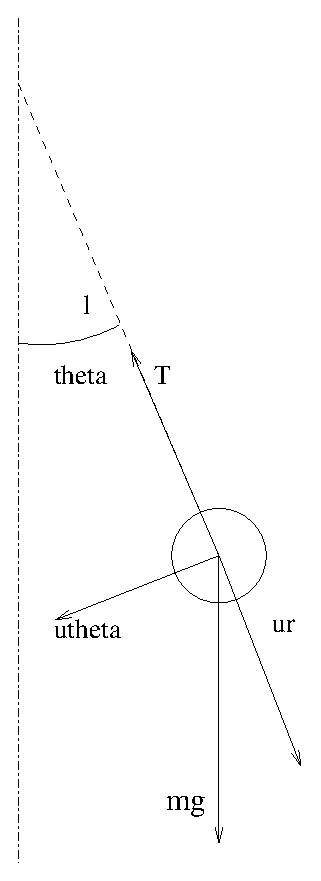
\includegraphics[scale=0.4]{immagini/fisica1/pendolo_forza}
  \caption{\index{pendolo}Pendolo semplice.}
\end{figure}
\[\ve F=m\ve g+\ve T=m\ve a\]
\[\left\{
  \begin{array}{l}
    a_r=-\frac{v^2}{l}=-\omega^2 l \\
    a_\theta=\frac{\ud v}{\ud t}
  \end{array}
  \right.\]
\[\left\{
  \begin{array}{l}
    mg\cos\theta-T=-m\omega^2l=-m\frac{v^2}{l} \\
    mg\sin\theta=\frac{\ud v}{\ud t}m
  \end{array}
  \right.\]
\[\omega=\frac{v}{l}=\frac{\ud\theta}{\ud t}\]
\[|v|=\omega l=l\frac{\ud\theta}{\ud t}\]
\[v=-l\frac{\ud\theta}{\ud t}\]
\[mg\sin\theta=-ml\frac{\ud^2\theta}{\ud t}\]
\[g\sin\theta=-l\frac{\ud^2\theta}{\ud t}\]
per piccole oscillazioni\footnote{è il primo sviluppo del polinomio di Taylor}: $\sin\theta\simeq\theta$
\[\frac{\ud^2\theta}{\ud t^2}=-\frac{g}{l}\theta\]
si noti che questa equazione altro non è che l'equazione di un oscillatore armonico\footnote{Questo succede sempre quando si considerano piccole oscillazioni nell'intorno di un punto di equilibrio stabile $x_0$:
\[
  m\ddot x \simeq \underbrace{F(x_0)}_0 + \left.\frac{\ud F}{\ud x}\right|_{x_0} (x-x_0) = k (x-x_0)
\]
con $\left.\frac{\ud F}{\ud x}\right|_{x_0}=k<0$ perché è un punto di equilibrio stabile.
}.
\[g\theta=-l\ddot\theta\qquad \theta=A\sin\left(\omega
  t+\varphi\right)\]
\[\theta=-\frac{l}{g}\,\ddot\theta\qquad\ddot\theta=-A\omega^2\sin\left(\omega
  t+\varphi\right)=-\omega^2\theta\]
\[\theta=-\frac{\ddot\theta}{\omega^2}\qquad \frac{1}{\omega^2}=\frac{l}{g}\qquad\omega^2=\frac{g}{l}\qquad\omega=\sqrt\frac{g}{l}\]
\[\theta=A\sin\left(\sqrt\frac{g}{l}\,t+\varphi\right)\]
\[2\pi+\sqrt\frac{g}{l}t+\varphi=\sqrt\frac{g}{l}(t+T)+\varphi\qquad
  \sqrt\frac{g}{l}T=2\pi\qquad
  T=2\pi\sqrt\frac{l}{g}=\frac{2\pi}{\omega}\]

\subsection{\index{forza!variabile!nella velocità}Forze variabili nella velocità}
Su un corpo in caduta agisce la forza di Stokes: $F_s=-\beta v$,
proporzionale alla velocità. $\beta$ dipende dalla viscosità del
mezzo e dalla geometria del corpo.

\[\ve F=m\ve g+\ve F_s=m\ve a\]
\[mg-F_s=ma\]
\[mg-\beta v=ma=m\frac{\ud v}{\ud t}\]
\[mg-\beta v=m\frac{\ud v}{\ud t}\qquad \ud t\left(mg-\beta v\right)=m\ud v\]
\[\int_0^t\ud t=\int_{v_0}^v\frac{m}{mg-\beta v}\,\ud v\]
\[t=\left[-\frac{m}{\beta}\ln\left(mg-\beta
    v\right)\right]_{v_0}^{v}=-\frac{m}{\beta}\left(\ln\left(mg-\beta
    v\right)-\ln\left(mg-\beta v_0\right)\right)=\]
\[=-\frac{m}{\beta}\ln\frac{mg-\beta v}{mg-\beta v_0}\qquad-\frac{\beta t}{m}=\ln\frac{mg-\beta v}{mg-\beta v_0}\]
\[e^{-\frac{\beta t}{m}}=e^{\ln\frac{mg-\beta v}{mg-\beta v_0}}=\frac{mg-\beta v}{mg-\beta v_0}\]
\[(mg-\beta v)=(mg-\beta v_0)e^{-\frac{\beta t}{m}}\]
\[v=\frac{mg}{\beta}\left(1-e^{-\frac{\beta
      t}{m}}\right)+v_0e^{-\frac{\beta t}{m}}\]

se $t\rightarrow +\infty$ allora $v\rightarrow\frac{mg}{\beta}$

se $\beta\rightarrow 0$ allora $v\rightarrow gt+v_0$
\begin{figure}[htbp]
  \centering
  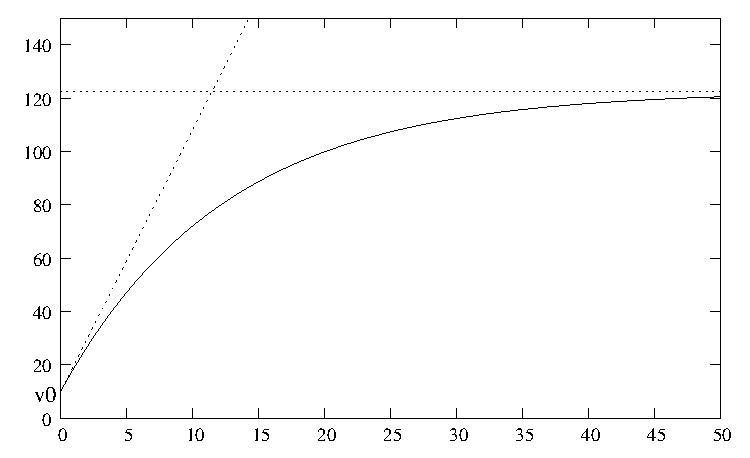
\includegraphics[scale=1]{immagini/fisica1/grafico_forze_nella_velocita}
  \caption{Grafico forza variabile nella velocità.}
\end{figure}

\section{\index{forza!apparente}Forze apparenti}
Le forze apparenti non sono delle vere forze, sono degli strumenti che consentono di usare la seconda legge delle dinamica anche in sistemi non inerziali. In particolare le forze apparenti non rispettano il terzo principio della dinamica.

\subsection{Sistema in moto lineare accelerato}
Con riferimento alla Figura~\ref{fig:forze_apparenti}, siano $O$ e $O'$ due sistemi di riferimento; sia $O$ un sistema inerziale e $O'$ si muova verso destra con accelerazione $\ve a_{O'}$ rispetto ad $O$. $\ve r_{O'}$ il vettore che individua $O'$ rispetto ad $O$. Possiamo scrivere le quantità cinematiche di un punto $P$ nel sistema di coordinate di $O$ rispetto a quelle di $O'$:
\[\ve r={\ve r}\,^\prime+\ve r_{O'}\qquad\ve v=\ve v\,'+\ve v_{O'}\qquad\ve a=\ve a\,'+\ve a_{O'}\]
\begin{figure}[tbp]
  \centering
  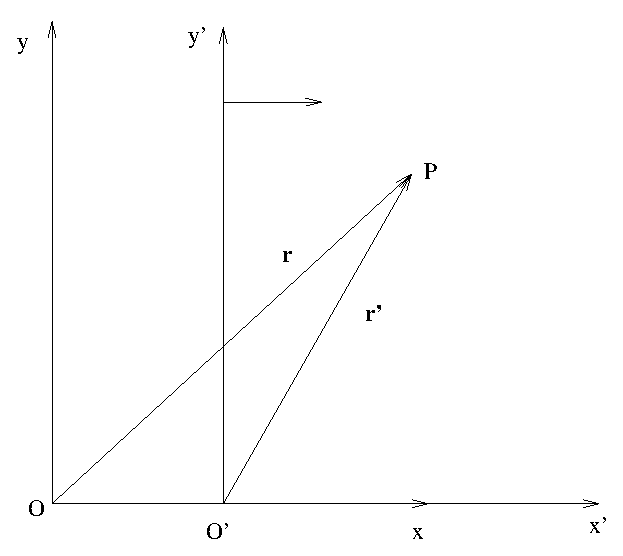
\includegraphics[scale=0.5]{immagini/fisica1/apparenti}
  \caption{Sistemi di riferimento in moto relativo}
  \label{fig:forze_apparenti}
\end{figure}
Se scriviamo il secondo principio della dinamica, che deve valere in generale solo nel sistema inerziale $O$:
\[m\ve a=m\ve a'+m\ve a_{O'}=\ve F\]
vediamo che questo non vale nel sistema $O'$ quando $a_O'\neq 0$:
\[m\ve a'=\ve F-m\ve a_{O'}=\ve F+\ve F_\text{app}\]
Possiamo però ritenere il secondo principio della dinamica valido in $O'$ se supponiamo che a causa dell'accelerazione del sistema, ci sia una forza apparente che agisca sui corpi:
\[\ve F_\text{app}=-m\ve a_{O'}\]
\subsection{Sistema in moto circolare uniforme (Terra)}
La Terra non è un sistema inerziale\index{sistema!inerziale}, infatti ruota intorno al Sole e ruota attorno al proprio asse. Consideriamo quest'ultimo moto con riferimento alla Figura~\ref{fig:forze_apparenti_terra}; siano $x'$ e $y'$ le coordinate di un punto viste dal sistema solidale con la Terra, mentre $x$ e $y$ quelle di un sistema inerziale. Si consideri la rotazione con velocità angolare $\omega$ costante. Dopo un certo tempo $t$, il sistema di riferimento della Terra, sarà ruotato di un angolo $\theta=\omega t$.
\begin{figure}[tbp]
  \centering
  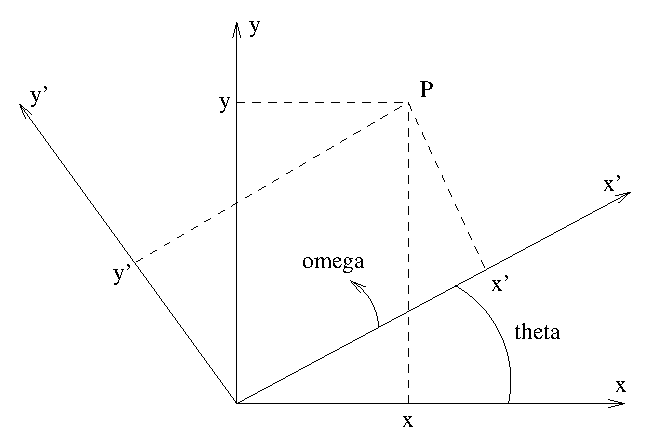
\includegraphics[scale=0.7]{immagini/fisica1/apparenti2}
  \caption{Sistema $O'$ in rotazione rispetto al sistema $O$.}
  \label{fig:forze_apparenti_terra}
\end{figure}

La componente lungo $x$ della velocità e dell'accelerazione del punto $P$ misurate da $O$ in funzione delle quantità misurate da $O'$:
\[\left\{\begin{array}{l}
    x(t)=x'(t)\cos(\omega t)-y'(t)\sin(\omega t) \\
    y(t)=y'(t)\cos(\omega t)+x'(t)\sin(\omega t)
  \end{array}\right.\]

\[v_x=\frac{\ud x}{\ud t}=v'_{x'}\cos\left(\omega t\right)-\omega x'\sin\left(\omega t\right)-v'_{y'}\sin\left(\omega t\right)-\omega y'\cos\left(\omega t\right)\]
\begin{align*}
  a_x= & \frac{\ud v_x}{\ud t}=a'_{x'}\cos\left(\omega t\right)-\omega v'_{x'}\sin\left(\omega t\right)-\omega v'_{x'}\sin\left(\omega t\right)-\omega^2 x'\cos\left(\omega t\right)- \\
       & -a'_{y'}\sin\left(\omega t\right)-\omega v'_{y'}\cos\left(\omega t\right)-\omega v'_{y'}\cos\left(\omega t\right)+\omega^2 y'\sin\left(\omega t\right)                       \\
  =    & a'_{x'}\cos\left(\omega t\right)-a'_{y'}\sin\left(\omega t\right)-\omega^2\left[x'\cos\left(\omega t\right)-y'\sin\left(\omega t\right)\right]-                              \\
       & -2\omega\left[v'_{x'}\sin\left(\omega t\right)+v'_{y'}\cos\left(\omega t\right)\right]                                                                                       \\
  =    & a'_{x}-\omega^2 x-2\omega v'_{y}
\end{align*}
\[\ve \omega\times\ve v'=\left|\begin{array}{ccc}
    \ve i   & \ve j   & \ve k   \\
    0       & 0       & \omega  \\
    v'_{x'} & v'_{y'} & v'_{z'} \\
  \end{array}
  \right|
  =-\omega v'_{y'}\ve i+\omega v'_{x'}\ve j\]

\[\left\{\begin{array}{l}
    a_x=a'_x-\omega^2 x+2\left(\ve \omega\times\ve v'\right)_x \\
    a_y=a'_y-\omega^2 y+2\left(\ve \omega\times\ve v'\right)_y \\
  \end{array}\right.\]

\[\ve a=\ve a'-\omega^2 \ve r+2\left(\ve\omega\times\ve v'\right)\]
\[m\ve a=m\ve a'-m\omega^2\ve r+2m\left(\ve\omega\times\ve v'\right)=\ve F\]
\[ma'=\ve F+\underbrace{m\omega^2\ve r}_\text{forza centrifuga}-\underbrace{2m\left(\ve\omega\times\ve v'\right)}_\text{forza di Coriolis}\]\index{Coriolis}\index{forza!centrifuga}\index{forza!di Coriolis}
\[\ve F_\text{cent}=m\omega^2 \ve r\qquad \ve F_\text{Cor}=-2m\left(\ve\omega\times\ve v'\right)\]

\begin{Es}[pendolo di Focault\index{Focault}\index{pendolo!di Focault}]
  Se mettiamo un pendolo al polo la forza centrifuga sarà nulla perché $r=0$, ma esiste ancora la forza di Coriolis. Sperimentalmente si osserva che il piano di rotazione del pendolo ruota a causa della non inerzialità della Terra.
\end{Es}
\subsection{Trattazione generale}
Siano $\{\ve{e}_i\}_i^3$ e $\{\ve{e}'_i\}_i^3$ i versori dei di due sistemi, $O$ e $O'$ e sia $O$ inerziale. Ogni vettore di $O$ si scrive come combinazione lineare i cui coefficienti sono le coordinate $\{x_i\}_i^3$:
\[
  \ve{x}=\sum_{i=1}^3 x_i\ve{e}_i
\]
sia $x_0$ il vettore posizione di $O'$ visto da $O$:
\[
  \ve{x_0}=\sum_{i=1}^3 {x_0}_i \ve{e}_i
\]
nella base del sistema $O'$ il punto individuato da $\ve x$ rispetto al sistema $O$ è individuato dal vettore $\ve{x'}$ e avrà velocità $\ve{v'}$:
\[
  \ve{x'}=\sum_{i=1}^3 x'_i\ve{e'}_i \qquad \ve{v'}=\sum_{i=1}^3 \frac{\ud x'_i}{\ud t}\ve{e'}_i
\]
La relazione che lega i vettori posizione è:
\[
  \ve{x} = \ve{x_0}+\ve{x'}
\]
ricaviamo la relazione che lega le velocità misurate dai sui sistemi:
\begin{equation}
  \ve{v}=\frac{\ud}{\ud t}\ve{x}=\frac{\ud}{\ud t}\ve{x_0}+\frac{\ud}{\ud t}\ve{x'}=\ve{v_0}+\sum_{i=1}^3\left(\underbrace{\frac{\ud x'_i}{\ud t}\ve{e}'_i}_{\ve{v'}}+x'_i\frac{\ud \ve{e}'_i}{\ud t}\right)
  \label{eq:forze_apperenti_gen_v}
\end{equation}
Si noti come $\ve v'\neq \ve{\dot x'}$, infatti:
\[
  \frac{\ud\ve x'}{\ud t} = \sum_{i=1}^3\left(\frac{\ud x'_i}{\ud t}\ve{e}'_i+x'_i\frac{\ud \ve{e}'_i}{\ud t}\right) = \ve{v'} + \sum_{i=1}^3 x'_i\frac{\ud \ve{e}'_i}{\ud t}
\]
Ricaviamo l'accelerazione vista da $O$:
\begin{equation}
  \begin{split}
    \ve{a} = \frac{\ud v}{\ud t} &= \ve{a_0}+\sum_{i=1}^3\left(\frac{\ud^2 x'_i}{\ud t^2}\ve{e}'_i
    +2\frac{\ud x'_i}{\ud t}\frac{\ud \ve{e}'_i}{\ud t}
    +x'_i\frac{\ud^2 \ve{e}'_i}{\ud t^2}\right) \\
    &= \ve{a_0} + \ve a'
    +2\sum_{i=1}^3 \frac{\ud x'_i}{\ud t}\frac{\ud \ve{e}'_i}{\ud t} + \sum_{i=1}^3 x'_i\frac{\ud^2 \ve{e}'_i}{\ud t^2}
  \end{split}
  \label{eq:fittizie_gen_a}
\end{equation}

Usando il secondo principio della dinamica $\ve F=m\ve a$ ricaviamo che nel sistema $O'$:
\begin{equation}
  m \ve{a'} = \ve F - m\ve{a_0}
  -2m \sum_{i=1}^3 \frac{\ud x'_i}{\ud t}\frac{\ud \ve{e}'_i}{\ud t} -m \sum_{i=1}^3 x'_i\frac{\ud^2 \ve{e}'_i}{\ud t^2}
  \label{eq:fittizie_gen_f}
\end{equation}
dove le ultime tre componenti sono forze fittizie.

Si definisce velocità di trascinamento\index{velocità!di trascinamento} la velocità misurata da $O$ di un punto fermo rispetto ad $O'$, cioè per cui $\ve v'=0$. Dalla \eqref{eq:forze_apperenti_gen_v}:
\begin{equation}
  \ve v_T = \ve{v_0}+\sum_{i=1}^3 x'_i\frac{\ud \ve{e}'_i}{\ud t}
  \label{eq:fittizie_gen_vt}
\end{equation}
La velocità di trascinamento è uguale alla differenza di velocità misurate dai due osservatori: $\ve v_T = \ve{v} - \ve{v'}$.
L'accelerazione di trascinamento è quella di un punto solidale con $O'$ misurata da $O$, quindi per questo punto $\ve v'=0$ e $\ve a'=0$. Dalla \eqref{eq:fittizie_gen_a}
\begin{equation}
  \ve a_T = \ve{a_0}
  +2\sum_{i=1}^3 \frac{\ud x'_i}{\ud t}\frac{\ud \ve{e}'_i}{\ud t} + \sum_{i=1}^3 x'_i\frac{\ud^2 \ve{e}'_i}{\ud t^2}
\end{equation}




\subsection{Casi particolari}
\subsubsection{Moto uniformemente accelerato}
Se $O'$ si muove di moto uniformemente accelerato allora in questo sistema di riferimento, dall'equazione~\eqref{eq:fittizie_gen_f}, la legge di Newton si scrive come :
\begin{equation}
  m\ve{a'} = \ve F - m\ve{a_0}
\end{equation}

\subsubsection{Moto rototraslatorio}
Consideriamo che il sistema $O'$ ruoti con velocità angolare $\omega$ e trasli con accelerazione $\ve a_0$ vista a $O$. A causa della rotazione il versore del sistema primato ruota, ma il suo modulo non cambia. Dopo un tempo $\ud t$ avrà fatto un angolo $\ud\alpha=\omega\ud t$, quindi per la definizione di angolo $\ud\alpha=\norm{\ud\ve{e'_i}}$. In generale vale:
\[
  \frac{\ud\ve{e'_i}}{\ud t}=\ve\omega\times\ve{e'_i}
\]
quindi dalla \eqref{eq:forze_apperenti_gen_v}:
\begin{equation}
  \ve{v}=\ve{v_0}+\ve{v'}+\ve{\omega}\times\ve{x'}
  \label{eq:forze_apparenti_rot_v}
\end{equation}
e la velocità di trascinamento dalla~\eqref{eq:fittizie_gen_vt}:
\[
  \ve v_T = \ve{v_0}+\ve{\omega}\times\ve{x'}
\]
L'accelerazione dalla~\eqref{eq:fittizie_gen_a}
\[
  \begin{split}
    \ve a &= \ve{a_0} + \ve a'
    +2\sum_{i=1}^3 \frac{\ud x'_i}{\ud t}(\ve\omega\times\ve{e'_i})+ \sum_{i=1}^3 x'_i\left(\frac{\ud\ve\omega}{\ud t}\times \ve{e'}_i + \ve\omega\times\frac{\ud\ve{e'}_i}{\ud t}\right) \\
    &= \ve{a_0} + \ve a'
    +2(\ve\omega\times\ve{v'})+ \frac{\ud\ve\omega}{\ud t}\times \ve{x'} + \ve\omega\times(\ve\omega\times \ve{x'}) \\
    &= \ve{a_0} + \ve a'
    +2(\ve\omega\times\ve{v'})+ \frac{\ud\ve\omega}{\ud t}\times \ve{x'} + \ve{\omega}(\ve\omega\cdot\ve{x'})-\ve{x'}(\ve\omega\cdot\ve\omega) \\
    & =\ve{a_0}+\ve{a'}+\frac{\ud\ve\omega}{\ud t}\times\ve x'+2\ve\omega\times\ve{v'}-\omega^2\ve{x'}
  \end{split}
\]
dove nel penultimo passaggio si è usato $\ve A\times(\ve B\times \ve C)=\ve{B}(\ve{A}\cdot\ve{C})-\ve{C}(\ve{A}\cdot\ve{B})$. Moltiplicando per $m$ si ottiene:
\begin{equation}
  \label{eq:newton_non_inerziale}
  m\ve{a'}=\ve F-m\ve{a_0}-m\frac{\ud\ve\omega}{\ud t}\times\ve x'+m\omega^2\ve x'-2m\ve\omega\times\ve{v'}
\end{equation}
Le forze fittizie che compaiono, oltre a $m\ve{a_0}$ sono la foze di Eulero\index{forza!di Eulero}, la forze centrifuga\index{forza!centrifuga} e la forza di Coriolis\index{forza!di Coriolis}.
L'accelerazione di trascinamento:
\[
  \ve a_T = \ve{a_0}+\frac{\ud\ve\omega}{\ud t}\times\ve x'-\omega^2\ve{x'}
\]
e quindi:
\[
  \ve a = \ve a'+\ve a_T + \underbrace{2\ve\omega\times\ve v'}_{\ve a_c}
\]
dove $\ve a_C$ è l'\index{accelerazione!di Coriolis}accelerazione di Coriolis.
\subsubsection{Moto circolare uniforme}
Per questo caso $\ve a_0=0$ e $\omega$ è costante:
\begin{equation}
  \ve F = m\ve a' + m\omega^2\ve x' - 2m\ve \omega \times\ve v'
\end{equation}
dove il primo termine addizionale è la \index{forza!centrifuga}forza centrifuga, mentre il secondo è la \index{forza!di Coriolis}forza di Coriolis.

\section{\index{quantità di moto}Quantità di moto}
\begin{Def}[quantità di moto di un punto materiale]
  \begin{equation}
    \ve{p}:=m\ve{v}
  \end{equation}
  sinonimi di quantità di moto sono: quantità di modo lineare, momento, momento lineare.
\end{Def}
La derivata della quantità di moto è la forza, ed è in questo modo che Newton introdusse il secondo principio:
\begin{equation}
\frac{\ud \ve p}{\ud t}=\frac{\ud\left(m\ve v\right)}{\ud t}=m\ve a=\ve F
\end{equation}
\subsection{Sistema di \texorpdfstring{$N$}{N} punti}
\begin{Def}[quantità di moto di un sistema di $N$ punti]
  La quantità di moto totale di un sistema di $N$ punti è la somma delle quantità di moto dei singoli punti.
  \begin{equation}
    \ve p=\sum_{I=1}^N\ve p_i
  \end{equation}
\end{Def}
\begin{Teo}
  La variazione della quantità di moto di un sistema è uguale alle forze esterne:
  \begin{equation}
    \frac{\ud \ve p}{\ud t}=\sum^N_{i=1}\stackrel{\text{Est}}{\ve F_i}
  \end{equation}
 Si conclude che in un sistema isolato, cioè con
  $\sum^N_{i=1}\stackrel{\text{Est}}{\ve F_i}=0$ vale la legge di
  conservazione della quantità di moto del sistema.
\end{Teo}
Consideriamo che su ogni punto agiscono sia forze esterne, che forze interne, cioè derivanti dall'interazione con altri punti del sistema:
\[
  \frac{\ud \ve p}{\ud t}  =\frac{\ud }{\ud t}\sum^N_{i=1}m_i\ve v_i=\sum_{i=1}^{N}m_i\ve a_i=
  =\sum^N_{i=1}\stackrel{\text{Est}}{\ve F_i}+\sum^N_{i=1}\stackrel{\text{Int}}{\ve F_i}=\sum^N_{i=1}\stackrel{\text{Est}}{\ve F_i}\]
Nell'ultimo passaggio abbiamo usato il terzo principio della dinamica $\stackrel{\text{Int}}{\ve{F_{ij}}} = -\stackrel{\text{Int}}{\ve{F_{ji}}}$:
\[
  \sum^N_{i=1}\stackrel{\text{Int}}{\ve F_i} = \sum_{i\neq j}\stackrel{\text{Int}}{\ve F_{ij}} = \frac{1}{2}\sum_{i\neq j}\left(\stackrel{\text{Int}}{\ve F_{ij}} + \stackrel{\text{Int}}{\ve{F_{ij}}}\right) = \frac{1}{2}\sum_{i\neq j}\stackrel{\text{Int}}{\ve{F_{ij}}} + \sum_{i\neq j}\stackrel{\text{Int}}{-\ve{F_{ji}}} = 0
  \]

\begin{Es}[decadimento]
  L'uranio decade in questo modo:
  \[\ce{^{238}_{92}U -> ^{234}_{90}Th + ^{4}_{2}\alpha}\]
  Consideriamo il sistema di riferimento in cui l'uranio è a riposo, quindi $\ve p_0=0$:
  \[\ve p_f=m_{\ce{Th}}\ve v_{\ce{Th}}+m_\alpha \ve v_\alpha=\ve p_0=0\]
  \[
    m_{\ce{Th}}v_{\ce{Th}}=m_\alpha v_\alpha\qquad v_\alpha=\SI{2E7}{\metre\per\second}
  \]
  \[
    v_{\ce{Th}}=\frac{m_\alpha v_\alpha}{m_{\ce{Th}}}=\SI{3.4E5}{\metre\per\second}
  \]
\end{Es}

\section{\index{centro di massa}Centro di Massa}
\begin{Def}[Centro di massa di $N$ punti]
  \begin{equation}\ve r_{CM}=\frac{\sum^N_{i=1}\left(\ve
    r_im_i\right)}{\sum^N_{i=1}m_i}=\frac{\sum^N_{i=1}\left(\ve
    r_im_i\right)}{M}\end{equation}
  \[x_{CM}=\frac{\sum^N_{i=1}\left(x_im_i\right)}{M} \qquad
    y_{CM}=\frac{\sum^N_{i=1}\left(y_im_i\right)}{M}\qquad
    z_{CM}=\frac{\sum^N_{i=1}\left(z_im_i\right)}{M}\]
\end{Def}
\[\ve v_{CM}=\frac{\ud \ve r_{CM}}{\ud t}=\frac{\sum^N_{i=1}\frac{\ud}{\ud t}\left(m_i\ve r_i\right)}{\sum^N_{i=1}m_i}=\frac{\sum^N_{i=1}\left(m_i\ve v_i\right)}{M}\]
\[M\ve v_{CM}={\sum^N_{i=1}m_i\ve v_i}=\ve p\]
\[\frac{\ud \ve p}{\ud t}=\frac{\ud}{\ud t}M\ve v_{CM}=M\ve a_{CM}=\sum^N_{i=1}\stackrel{\text{Est}}{\ve F_i}\]
\begin{Teo}
  \begin{eqimp}{equation}
    M\ve V_{CM}=\ve P \qquad M\ve a_{CM}=\sum \stackrel{\text{Est}}{\ve F_i}
  \end{eqimp}
  Se il sistema è isolato $\sum \stackrel{\text{Est}}{\ve F}=0$
  \[M\ve a_{CM}=0 \Rightarrow \ve a_{CM}=0\]
  allora il centro di massa si muove di moto rettilineo uniforme.
\end{Teo}

\subsection{Corpo continuo}
\begin{Def}[Centro di massa per un corpo continuo]
  \begin{equation}\ve r_{CM}=\frac{\int_V \ve r\,\ud m}{M}\end{equation}
\end{Def}
\begin{Def}[Densità media]
  \begin{equation}\rho =\frac{m}{V}\end{equation}
\end{Def}
\begin{Def}[Densità locale]
  \begin{equation}\rho(x,y,z)=\frac{\ud m}{\ud V}\end{equation}
\end{Def}
\[\ud m=\rho\,\ud V\]
\[M=\int_V \ud m=\int_V\rho \,\ud V\]
\begin{equation}\ve r_{CM}=\frac{\int_V \ve r \ud V\rho}{M}=\frac{\int_V\rho\ve r\,\ud V}{\int_V \rho \,\ud V}\end{equation}
Se la densità è uguale in tutti i punti il centro di massa è solo un fattore geometrico:
\[\ve r_{CM}=\frac{\int_V\ve r\,\ud V}{V}\]

\begin{Es}[semicirconferenza]
  \label{es:semicirconferenza}
  \begin{figure}[htp]
    \centering
    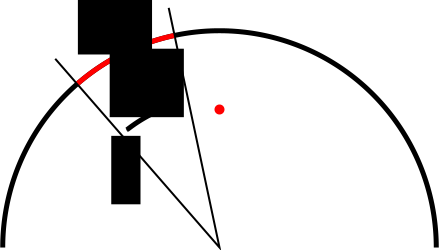
\includegraphics[scale=0.4]{immagini/fisica1/semicerchio}
    \caption{Esempio \ref{es:semicirconferenza}.}
  \end{figure}

  \[x_{CM}=0 \quad\text{per simmetria}\]
  \[\frac{\ud m}{M}=\frac{\ud s}{\pi r}\qquad \ud s=r\ud\theta\]
  \[\ud m=\frac{M\ud s}{\pi r}=\frac{Mr\ud\theta}{\pi r}=\frac{M\ud\theta}{\pi}\]
  \[y=r \sin \theta\]
  \[y_{CM}=\frac{\int y\ud m}{M}=\frac{r}{\pi}\int_0^\pi \sin\theta \ud \theta=-\frac{r}{\pi}\left[\cos\theta\right]_0^\pi=-\frac{r}{\pi}(-1-1)=\frac{2r}{\pi}\]
\end{Es}

\begin{Es}[cerchio bucato]
  \label{es:cerchio_bucato}
  \begin{figure}[htp]
    \centering
    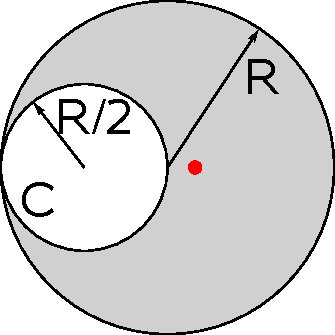
\includegraphics[scale=0.7]{immagini/fisica1/luna}
    \caption{Esempio \ref{es:cerchio_bucato}.}
  \end{figure}

  Luna è il cerchio grande meno il piccolo ($C$) di raggio
  $\frac{r}{2} \quad y_{CM}=0$ per simmetria
  \[M^C=\rho\pi\left(\frac{r}{2}\right)^2=\rho\pi\left(r^2-\frac{r^2}{4}\right)=\frac{3}{4}\rho\pi r^2\qquad M^{\text{luna}}=\rho\left(\pi r^2-\pi\left(\frac{r}{2}\right)^2\right)\]
  \[x_{CM}^{\text{pieno}}=0=\frac{x_{CM}^{\text{luna}}+x_{CM}^CM^C}{M^C+M^{\text{luna}}}\]
  \[0=x_{CM}^{\text{luna}}x_{CM}^C\frac{M^C}{M^{\text{luna}}}=x_{CM}^{\text{luna}}x_{CM}^C\frac{4M^C}{3\rho \pi r^2}=x_{CM}^{\text{luna}}x_{CM}^C\frac{4\rho\pi r^2}{4\cdot 3\rho\pi r^2}=\frac{x_{CM}^{\text{luna}}x_{CM}^C}{3}\]
  \[x_{CM}^{\text{luna}}=3x_{CM}^C=\frac{R}{6}\]
\end{Es}

\subsection{\index{teorema!di Pappo--Guldino}Teorema di Pappo--Guldino}
\begin{Teo}[Pappo--Guldino]
  Il volume generato dalla rotazione di una superficie è uguale
  all'area della superficie per la distanza percorsa dal centro di
  massa durante la rotazione.
\end{Teo}
\begin{Es}[Semicerchio]
  Il volume generato dalla rotazione del semicerchio è il volume della
  sfera: $\frac{4}{3}\pi r^3$, la distanza percorsa dal centro di
  massa è $2\pi y$ con $y$ l'ordinata del centro di massa, la
  superficie del semicerchio è $\frac{\pi r^2}{2}$, quindi
  \[2\pi y\frac{\pi r^2}{2}=\frac{4}{3}\pi r^3\]
  \[y=\frac{4}{3\pi}r\]
\end{Es}

\section{\index{impulso di una forza}Impulso di una forza}
\begin{Def}[Impulso di una forza]
  L'impulso di una forza $\ve F$ tra il tempo $t_1$ e $t_2$ è definito come:
  \begin{equation}
    \ve{J}(t_1,t_2)=\int_{t_1}^{t_2} \ve{F}\, \ud t
  \end{equation}
\end{Def}
poiché
\begin{align*}
  \int_{t_1}^{t_2} \ve{F}\, \ud t & = \int_{t_1}^{t_2}m\ve a\, \ud t=m\int_{\ve v(t_1)}^{\ve v(t_2)}\frac{d\ve{v}}{\ud t}\,\ud t=m\int_{t_1}^{t_2}\ud \ve{v} \\
                                  & =m\left[\ve v(t_2)-\ve v(t_1)\right]=\ve p_2 - \ve p_1=\Delta \ve p
\end{align*}
allora:
\begin{Teo}[inpulso]
  \[
    \ve J=\int_{t_1}^{t_2}\ve F \ud t=\Delta \ve p
  \]
\end{Teo}
In particolare se il sistema è isolato con due corpi si ha:

\[
  \Delta \ve p_1=\int_{t_1}^{t_2} \ve F_{1,2}\, \ud t\qquad \Delta \ve p_2=\int_{t_1}^{t_2} \ve F_{2,1}\, \ud t
\]
\[
  \Delta \ve p_1 + \Delta \ve p_2=\int\left(\ve F_{1,2}+\ve F_{2,1}\right)\ud t=0=\Delta\ve p_{\text{totale}}
\]
\[
  \ve p_{\text{iniziale}}=\ve p_{\text{finale}}
\]
dove si è usato terzo principio della dinamica. La conservazione della quantità di moto vale in tutti i sistemi isolati.

\section{\index{urti}Urti}
Gli urti si classificano in elastici ed anelastici. Gli urti reali sono una via intermedia. Negli urti elastici si conserva tutta l'energia cinetica, agiscono solo forze conservative; durante l'urto l'energia cinetica si trasforma in energia potenziale, per poi tornare completamente energia cinetica. La quantità di moto si conserva sempre in quanto non agiscono forze esterne.

\subsection{\index{urti!elastici}Urti elastici}

\subsubsection{Urti in 1 dimensione}

\[ \left \{
  \begin{array}{ll}
    m_1v_{i,1}+m_2v_{i,2}=m_1v_{f,1}+m_2v_{f,2}                                                     & v_{1,f}=? \\
    \frac{1}{2}m_1v_{i,1}^2+\frac{1}{2}m_2v_{i,2}^2=\frac{1}{2}m_1v_{f,1}^2+\frac{1}{2}m_2v_{f,2}^2 & v_{2,f}=?
  \end{array}
  \right.\]
\[v_{1,f}=\frac{2m_2}{m_1+m_2}v_{i,2}-v_{i,1}\frac{m_2-m_1}{m_1+m_2}\]
\[v_{2,f}=\frac{2m_1}{m_1+m_2}v_{i,1}-v_{i,2}\frac{m_1-m_2}{m_1+m_2}\]

\subsubsection{casi limite}
\label{casilimiteurti}
\begin{enumerate}
  \item $m_1=m_2$
        \[v_{f,1}=v_{i,2}\]
        \[v_{f,2}=v_{i,1}\]
        \begin{itemize}
          \item $v_{i,2}=0$
                \[v_{f,1}=0\]
                \[v_{f,2}=v_{i,1}\]
        \end{itemize}
  \item $m_2\gg m_1$
        \[\frac{m_1}{m_2}\simeq 0\]
        \[v_{f,1}=-v_{i,1}+2v_{i,2}\]
        \[v_{f,2}=v_{i,2}\]
        \begin{itemize}
          \item $v_{i,2}=0$
                \[v_{f,1}=-v_{i,1}\]
                \[v_{f,2}=v_{i,2}=0\]
          \item $v_{i,1}=0$
                \[v_{f,1}=2v_{i,2}\]
                \[v_{f,2}=v_{i,2}\]
        \end{itemize}

\end{enumerate}

\subsubsection{Urti in due dimensioni}
Due corpi di massa $m_1$, $m_2$, prima dell'urto velocità $\ve v_{i,2}=0$, $\ve v_{i,1}$, il secondo corpo è fermo, dopo l'urto velocità $\ve v_{f,1}$, $\ve v_{f,2}$.

\[\left\{
  \begin{array}{l}
    m_1\ve v_{i,1}=m_1\ve v_{f,1}+m_2\ve v_{f,2} \\
    \frac{1}{2}m_1 v_{i,1}^2=\frac{1}{2}m_1 v_{f,1}^2+\frac{1}{2}m_2
    v_{f,2}^2
  \end{array}\right.\]

\[\left\{
  \begin{array}{l}
    m_1v_{i,1}=m_iv_{f,1}\cos\varphi_1+m_2v_{f,2}\cos\varphi_2 \\
    0=m_1v_{f,1}\sin\varphi_1-m_2v_{f,2}\sin\varphi_2          \\
    \frac{1}{2}m_1 v_{i,1}^2=\frac{1}{2}m_1 v_{f,1}^2+\frac{1}{2}m_2
    v_{f,2}^2
  \end{array}\right.\]
Il sistema è formato da 3 equazioni, ma da 4 incognite
($\varphi_1, \varphi_2, v_{f,1}, v_{f,2}$), ha $\infty^1$
soluzioni.

Nel caso particolare di $m_1=m_2$ si ha:
\[\frac{1}{2}m v_{i,1}^2=\frac{1}{2}m
  v_{f,1}^2+\frac{1}{2}m v_{f,2}^2\]
\[\left\{
  \begin{array}{l}
    v_{i,1}^2=v_{f,1}^2+v_{f,2}^2 \\
    m^2v_{i,1}^2=m^2v_{f,1}^2+m^2v_{f,2}^2+2m^2v_{1,f}v_{2,f}\cos\alpha
  \end{array}
  \right.\]

\[\left\{
  \begin{array}{l}
    v_{i,1}^2=v_{f,1}^2+v_{f,2}^2 \\
    v_{i,1}^2=v_{f,1}^2+v_{f,2}^2+2v_{1,f}v_{2,f}\cos\alpha
  \end{array}
  \right.\]

quindi $\cos \alpha=0\quad\Rightarrow\quad\alpha=\SI{90}{\degree}$, oppure $v_{1,f}=0$ e $v_{2,f}=v_{1,i}$

\subsection{\index{urti!anelastici}Urti completamente anelastici}

Negli urti anelastici il sistema perde la massima energia cinetica possibile, che non è tutta
in quanto se il sistema perdesse tutta l'energia cinetica violerebbe la conservazione
della quantità di moto. Si dimostra che questo caso è quello in cui dopo l'urto i due corpi
rimangono attaccati.

\begin{Es}[pendolo balistico{\index{pendolo!balistico}}]
  Un proiettile di massa $m$, velocità $v$ urta un pendolo balistico di massa $M>m$ e velocità $V=0$. Prima dell'urto la quantità di moto totale del sistema è $mv$, dopo $(M+m)V$.
  \[mv=(M+m)V\]
  \[V=\frac{mv}{M+v}\]
  Dopo l'urto il pendolo balistico, con il proiettile incorporato oscilla come un pendolo, l'energia meccanica si conserva, quindi $K_A=U(B)$


  \[\frac{1}{2}(m+M)V^2=(m+M)gh\]
  \[\frac{1}{2}\left(\frac{mv}{M+m}\right)^2=(m+M)gh\]
  \[\frac{1}{2}\frac{m^2v^2}{M+m}=(m+M)gh\]
  \[v^2=\frac{(m+M)gh\cdot 2(m+M)}{m^2}=\frac{2(m+M)^2gh}{m^2}\]
  \[v=\frac{m+M}{m}\sqrt{2gh}\]
  Consideriamo un sistema di riferimento $\ast$ inerziale rispetto
  al CM con la stessa velocità del CM.

  \[\ve P^\ast_{\text{prima}}=(m+M)\ve V_{\text{CM}}^\ast=0\]
  \[\ve P^\ast_{\text{dopo}}=0\quad\text{sono attaccati}\quad \ve
    v=0\] Quindi tutta l'energia cinetica è persa.
\end{Es}
\section{\index{momento!d'inerzia}Momento d'inerzia}
Corpo rigido(CR): presi due punti qualsiasi la loro distanza
rimane inalterata. Servono tre punti, quindi 9 coordinate, ma le
distanze rimangono fisse nel tempo, quindi il corpo ha 6 gradi di
libertà. Per descrivere il moto di un corpo bisogna dare 6
coordinate in funzione del tempo. Se fissiamo un asse di rotazione
si ha un solo grado di libertà. In questo caso si ha una rotazione
intorno ad un asse fisso. Ogni punto del CR descrive una
circonferenza. $\theta$ è comune a tutti, quindi anche $\omega$ e
$\alpha$
\[\ud s_i=\ud \theta r_i\]
\[v_i=r_i\omega \qquad a_t=\frac{\ud v_i}{\ud t}=\alpha r_i\]
\[K=\sum_i\frac{1}{2}m_iv_i^2\]
\[K=\sum_i\frac{1}{2}m_i\omega^2r_i^2=\frac{1}{2}\omega^2\left(\sum_im_ir_i^2\right)=\frac{1}{2}I\omega^2\]
\[I=\text{momento d'inerzia}=\sum_{i=1}^N m_ir_i^2\]
\[\text{Nel caso di corpo continuo} \sum_{i=1}^\infty \ud m_ir_i^2=\int_V  r^2\,\ud m\]
Essendo $\ve r$ relativo a un punto $O$ allora anche $I$ sarà relativo ad $O$. Bisogna sempre specificare rispetto quale punto si calcola $I$.

\subsection{Calcolo Momenti di Inerzia}

\begin{minipage}[c]{\textwidth}
  \subsubsection{Barra Sottile per l'estremo}

  \centering
  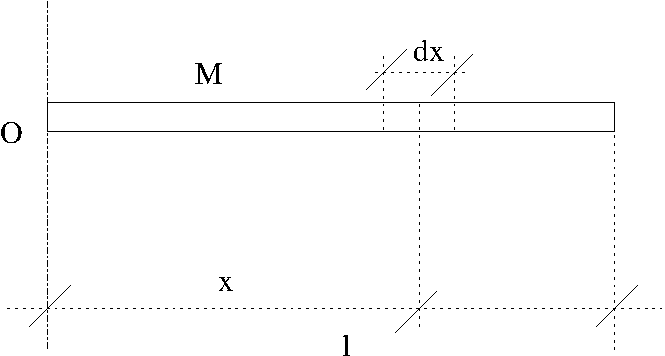
\includegraphics[scale=0.4]{immagini/fisica1/sbarra_sottile1}

  \[\frac{\ud m}{M}=\frac{\ud x}{l}\]
  \[I_0=\int_0^l\frac{M}{l}\ud x x^2=\frac{M}{l}\left[\frac{x^3}{3}\right]_0^l=\frac{M}{l}\frac{l^3}{3}=\frac{M}{3}l^2\]
\end{minipage}

\subsubsection{Barra sottile per il centro di massa}
\[I_c=\int_{-l/2}^{l/2}\frac{M}{l}\ud x
  x^2=\frac{M}{l}\int_{-l/2}^{l/2}x^2 \ud
  x=\frac{M}{3l}\left(\frac{l^3}{8}+\frac{l^3}{8}\right)=\frac{M}{12}l^2\]

\subsubsection{Disco}


\begin{figure}[htbp]
  \centering
  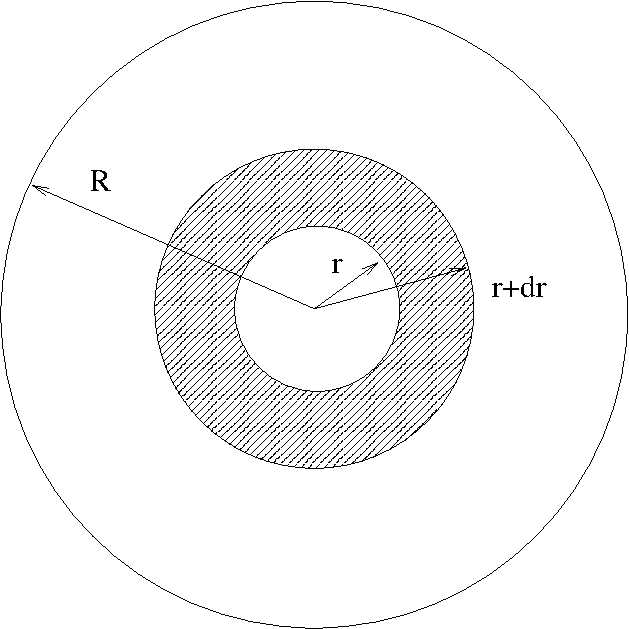
\includegraphics[scale=0.3]{immagini/fisica1/disco}
\end{figure}

\[\frac{\ud m}{M}=\frac{2\pi r\ud r}{\pi R^2}\]
\[\ud m=M\frac{2\ud r}{R^2}r\]
\[I_O=\int_O^R\frac{M}{R^2}2\ud r r^3=\frac{2M}{R^2}\int_O^R r^3
  \ud r=\frac{2M}{R^2}\cdot\frac{R^4}{4}=\frac{1}{2}MR^2\]

\subsubsection{Sfera omogenea}

\begin{minipage}[]{\textwidth}
  Dividiamo la sfera in tanti dischetti:
  \vspace{0.7cm}

  \centering
  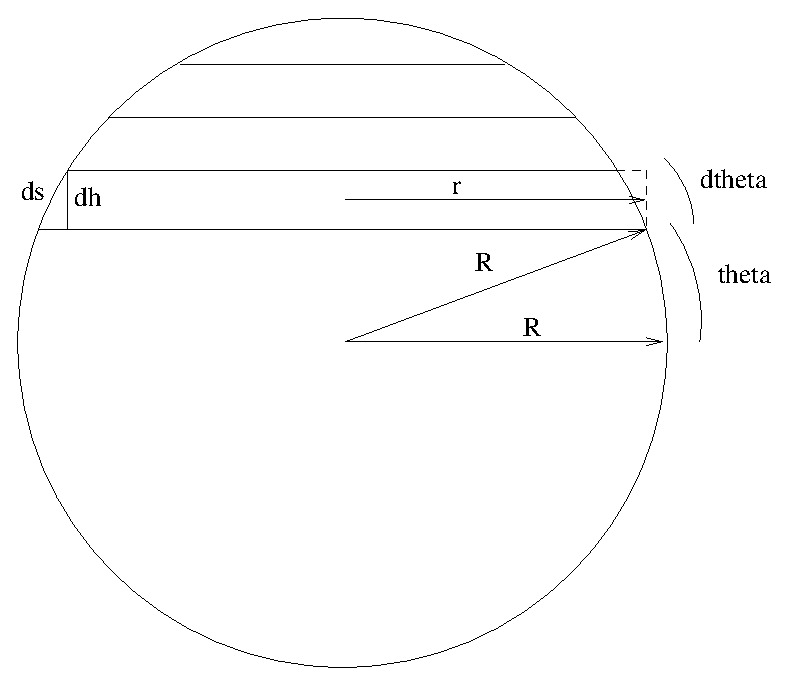
\includegraphics[scale=0.45]{immagini/fisica1/sfera_omogenea1}

\end{minipage}
\[r=R\cos\theta\quad \ud s=R\ud\theta\quad \ud h=\ud s\cos\theta=R\ud\theta\cos\theta\]
\[\ud m=\rho\ud V=\rho\pi r^2\ud h=\rho\pi R^2\cos^2\theta R\cos\theta\ud\theta=R^3\rho\pi\cos^3\theta\ud\theta\]
\[I_\text{dischetto}=\ud I=\frac{1}{2}\ud m r^2=\frac{1}{2}\rho\pi R^3\cos^3\theta\ud\theta R^2\cos^2\theta=\frac{1}{2}\rho\pi R^5\cos^5\theta\ud\theta\]
\[m=\rho\frac{4}{3}\pi R^3\]
\[I_\text{sfera}=2\int_0^\frac{\pi}{2}\ud I=\frac{3}{4}mR^2\int_0^\frac{\pi}{2}\cos^5\theta\ud\theta=\frac{2}{5}mR^2\]

\subsection{\index{teorema!di Steiner}\index{teorema!degli assi paralleli}Teorema di Steiner o degli assi paralleli}
\begin{Teo}[Steiner o degli assi paralleli]Sia $d$ la distanza da un asse di rotazione $I_0$ parallelo all'asse $I_{CM}$ passante per il centro di massa. Allora:
  \[I_0=d^2M+I_{CM}\]
\end{Teo}
\begin{figure}[htbp]
  \centering
  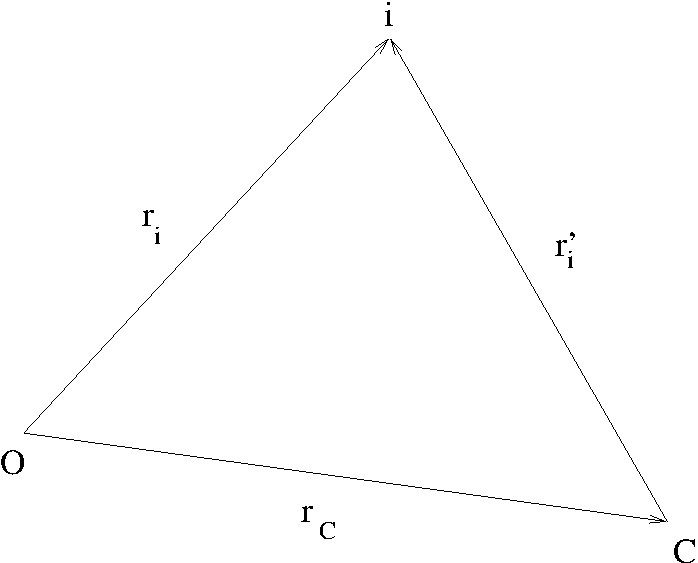
\includegraphics[scale=0.45]{immagini/fisica1/steiner}
\end{figure}
\[\ve r_i=\ve r_C+\ve r_i\,'\]
\[\ve r_i\cdot\ve r_i=r_i^2=\left(\ve
  r_C+r_i\,'\right)\cdot\left(\ve r_C+\ve r_i\,'\right)\Rightarrow
  r_i^2=r_C^2+r_i\,'^2+2\ve r_C\cdot\ve r_i\,'\]
\begin{align*}
  I_0 & =\sum m_ir_i^2=\sum r_C^2m_i+\sum r_i\,'^2m_i+\sum m_i
  \cdot 2\ve r_C\cdot \ve r_i\,'                               \\
      & =r_C^2\sum m_i+I_C+2\ve
  r_C\cdot\sum m_i\ve r_i\,'=d^2M+I_{C}+2\ve r_C\cdot\sum m_i\cdot
  \ve r_i\,'\end{align*}
Per ipotesi $C$ è il $CM$ del sistema
\[I_0=d^2 M+I_{CM}+2\ve r_i\frac{\sum m_i\ve r_i\,'}{M}\cdot
  M=d^2M+I_{CM}+2\ve r_i\cdot \ve r\,_{CM}^{CM} M=d^2M+I_{CM}\]
Ma $Md^2>0$ quindi $I_{CM}$ è il momento minimo possibile.
\begin{Es}
  Il momento d'inerzia di una circonferenza rispetto al centro di massa è \mbox{$I_{CM}=\frac{1}{2}MR^2$}, per un estremo è:
  \[I_0=I_{CM}+MR^2=\frac{1}{2}MR^2+MR^2=\frac{3}{2}MR^2>I_{CM}\]
\end{Es}
\section{\index{momento!di una forza}Momento di una forza}
\begin{Def}[Momento di una forza]
  Il momento di una forza (o momento torcente) rispetto ad un polo fisso $O$
  \begin{equation}
    \ve{\tau}_O=\ve r \times \ve F
  \end{equation}
  dove $\ve r$ è il vettore che individua il punto di applicazione dela forza rispetto al polo.
\end{Def}
\[\delta L=\ud K\qquad \ud \ve s=\ve r\ud \theta\]
\[\delta L=F\ud s\cos \phi=Fr\ud\theta\cos\phi\]
\[K=\frac{1}{2}I\omega^2\qquad\ud K=I\omega\ud\omega\]
\[Fr\ud\theta\cos\phi=I\omega\ud\omega\]
\[Fr\frac{\ud\theta}{\ud t}\cos\phi=I\omega\frac{\ud\omega}{\ud
    t}\]
\[Fr\omega\cos\phi=I\omega\alpha\]
\[Fr\cos\phi=I\alpha\]
\[Fr\sin\beta=I\alpha\]
\[\ve\tau=I\ve\alpha\qquad\text{analoga a $\ve F=m\ve a$}\]
\section[\index{momento!angolare}\index{momento!della quantità di moto}Momento angolare o della quantità di moto]{Momento angolare\\ o momento della quantità di moto}
\[\ve l_0=\ve r\times m\ve v\qquad\text{rispetto al polo $0$ fisso.}\]
\begin{align*}
  \frac{\ud \ve l_0}{\ud t} & =\frac{\ud}{\ud t}\left(\ve r\times m\ve v\right)= \frac{\ud\ve r}{\ud t}\times m\ve v+\ve r\times\frac{\ud m\ve v}{\ud t} \\
                            & =\ve v\times m\ve v+\ve r \times m\ve a=\ve r\times m\ve a=\ve r\times\ve F=\ve \tau_0
\end{align*}
\[\frac{\ud\ve l_0}{\ud t}=\ve \tau_0\qquad\text{analoga
    a}\qquad\frac{\ud \ve p}{\ud t}=\ve F\]
\subsection{Sistema di N punti}
\[\ve L_0=\sum_{i=1}^N \ve l_{0_i}\]
\begin{align*}\frac{\ud \ve L_0}{\ud t} & =\sum_{i=1}^{N}\frac{\ud \ve l_{0_i}}{\ud
                t}=\sum_{i=1}^{N}\frac{\ud}{\ud t}\left(\ve r_i \times \ve
              v_i\right)=\sum_{i=1}^{N}\ve v_i\times m_i \ve v_i+\ve
              r_i\times m_i\ve a_i                                                  \\
                                        & =\sum_{i=1}^{N}\ve r_i\times m_i\ve
              a_i=\sum_{i=1}^{N}\ve r_i\times\ve F_i                                \\
                                        & =\sum_{i=1}^{N}\ve
              r_i\times\stackrel{\text{Int}}{\ve F_i}+\sum_{i=1}^{N}\ve
              r_i\times\stackrel{\text{Est}}{\ve F_i}=\sum_{i=1}^{N}\ve
              r_i\times \stackrel{\text{Est}}{\ve
                F_i}=\sum_{i=1}^{N}\stackrel{\text{Est}}{\ve \tau_0}\end{align*}
\subsubsection{Dimostrazione $\stackrel{\text{Int}}{\ve\tau_0}=0$}
\[\ve F_{1,2}=-\ve F_{2,1}\]
\[\ve r_1\times \ve F_{1,2}+\ve r_2\times\ve F_{2,1}=\ve r_1\times \ve F_{1,2}-\ve r_2\times\ve F_{1,2}=\left(\ve r_i-\ve r_2\right)\times\ve F_{1,2}=0\]
perché $\left(\ve r_1-\ve r_2\right)\parallel \ve F_{1,2}$
\subsection{Conservazione del momento angolare}
Se il sistema è isolato si ha: $\stackrel{\text{Est}}{\ve
    F}=0\Rightarrow \stackrel{\text{Est}}{\ve \tau}=0$
\[\frac{\ud \ve L_0}{\ud t}=\ve \tau_0=0\qquad \ve
  L_0=\overrightarrow{\const}\]
e quindi
$I\omega={\const}$. Tutto ciò per la simmetria per
rotazioni.
\subsection{Rotazione intorno a \texorpdfstring{$O'$}{O'} mobile}
\[\ve r_i=\ve r_{O'}+\ve r_i\,'\qquad \ve r_i\,'=\ve r_i-\ve r_{O'}\]
\[L_{O'}=\sum\ve r_i\,'\times m\ve v_i=\sum(\ve r_i-\ve
  r_{O'})\times m\ve v_i\]
\begin{align*}
  \frac{\ud L_{O'}}{\ud t} & =\sum(v_i-v_{O'})\times m\ve v_i+r_i\,' m\ve a_i=-\sum\ve v_{O'}\times m_i\ve v_i+\sum\ve r_i\,'\times\ve F_i \\
                           & =\ve v_{O'}\times\sum m_i\ve v_i+\ve \tau_{O'}=-\ve
  v_{O'}\times\ve P+\stackrel{\text{Est}}{\tau_{O'}}
\end{align*}
\[\frac{\ud L_O}{\ud t}=-\ve v_{O'}\times\ve P+\stackrel{\text{Est}}{\tau_{O'}}\]

se $v_{O'}=0$ allora $-v_{O'}\times\ve P=0$

se $O'=CM$ allora $M\ve V_{CM}=\ve p\Rightarrow\ve
  v_{CM}\parallel\ve P\Rightarrow -\ve v_O\times\ve P=0$

\subsection{Rotazione intorno ad un asse}
\[\ve l_i=\ve r_i\times m_i\ve v_i\]
\[l_{i_z}=|\ve l_i|\sin\theta_i\]
\[|\ve l_i|=r_im_iv_i\qquad l_{i_z}=r_im_iv_i\sin\theta_i\qquad
  \omega d_i=v_i\]
\[l_{i_z}=m_id_i\omega d_i=md_i^2\omega\]
\[l_{i_z}=m_i\omega R_i^2\]
\[L_z=\sum l_{i_z}=\sum(m_id_i^2)\omega=I\omega\]
\[L_z=I\omega\]
\[\frac{\ud l_{i_z}}{\ud t}=I\frac{\ud \omega}{\ud
    t}=I\alpha\qquad \stackrel{\text{Est}}{\tau_{z}}=I\alpha\]
\subsection{Corpo simmetrico rispetto all'asse di rotazione}
\[\ve l_i+\ve l_{i'}=\alpha\ve k\]
\[L=I\omega=L_z\]


\section{Analogia tra grandezze lineari e \mbox{rotazionali}}
\begin{small}
  \begin{tabular}{p{4.0cm}p{2.45cm}p{4.0cm}p{2.38cm}}
    \hline
    Grandezze lineari                                 &                                                                                                                     & Grandezze rotazionali                                 &                              \\
    \hline
    velocità                                          & $\ve v=\ud \ve r/\ud t$                                                                                             & velocità angolare                                     & $\ve\omega=\ud \phi/\ud t$   \\
    Accelerazione                                     & $\ve a=\ud \ve v/\ud t$                                                                                             & Accelerazione
    angolare                                          & $\ve\alpha=\ud \ve\omega/\ud t$                                                                                                                                                                            \\
    Massa                                             & $m$                                                                                                                 & Momento d'inerzia                                     & $I=\sum mr^2$                \\
    Forza                                             & $\ve F$                                                                                                             & Momento di una forza                                  & $\ve \tau=\ve r\times \ve F$ \\
    Seconda legge di Newton                           & $\sum \stackrel{\text{Est}}{\ve F}=m\ve
    a$                                                & Seconda legge di Newton per moto rotatori con asse
    fisso                                             & $\sum\stackrel{\text{Est}}{\ve \tau_z}=I\alpha_z$                                                                                                                                                          \\
    Condizione di equilibrio                          & $\sum\stackrel{\text{Est}}{\ve
    F}=0$                                             & Condizione di equilibrio                                                                                            & $\sum\stackrel{\text{Est}}{\ve
    \tau}=0$                                                                                                                                                                                                                                                       \\
    quantità di moto di una particella                & $\ve p=m\ve v$                                                                                                      & Momento
    angolare di una particella                        & $\ve l=\ve r\times \ve p$                                                                                                                                                                                  \\
    quantità di moto di un sistema di particelle      & $\ve P=M\ve
    v_{CM}$                                           & Momento angolare di un sistema di particelle                                                                        & $\ve
    L=I\omega$                                                                                                                                                                                                                                                     \\
    Forma generale della seconda legge di
    Newton                                            & $\sum\stackrel{\text{Est}}{\ve F}=\ud \ve P/\ud t$                                                                  & Forma
    generale della seconda legge di Newton per i moti
    rotatori                                          & $\sum\stackrel{\text{Est}}{\ve \tau}=\ud \ve L/\ud t$                                                                                                                                                      \\
    Conservazione della quantità di moto di un sistema di particelle
    per il quale $\sum\stackrel{\text{Est}}{\ve F}=0$ & $\ve P=\sum
    \ve p_n=$ \mbox{$=\overrightarrow\const$}         & Conservazione del momento angolare di un sistema di particelle per il quale $\sum\stackrel{\text{Est}}{\ve \tau}=0$ & $\ve L=\sum \ve l_n=$ \mbox{$=\overrightarrow\const$}                                \\
    \hline
  \end{tabular}
\end{small}